% !TEX program = tectonic
\documentclass[11pt,a4paper]{article}
\usepackage[margin=22mm,headheight=14pt]{geometry}
\usepackage[T1]{fontenc}
\usepackage{lmodern}
\usepackage{microtype}
\usepackage{graphicx}
\usepackage{booktabs,longtable,tabularx,array}
\usepackage{amsmath,amssymb}
\usepackage{cite}
\usepackage{enumitem}
\usepackage{caption}
\usepackage{pdflscape}
\usepackage{fancyhdr}
\usepackage{hyperref}
\hypersetup{colorlinks=true,linkcolor=blue,citecolor=blue,urlcolor=blue}
\setlength{\parskip}{0.42em}
\setlength{\emergencystretch}{3em}
\setlength{\parindent}{0pt}
\pagestyle{fancy}
\fancyhf{}
\lhead{VLSI System Design Lab}
\rhead{4-bit Ripple-Carry Adder}
\cfoot{\thepage}
\newcommand{\StudentList}{\begin{tabular}{c}Saksham Arora \textbar\ 24BEC0185\\[2pt]Devansh Pandey \textbar\ 24BEC0312\\[2pt]Anand Menon \textbar\ 24BEC0444\end{tabular}}
\newcommand{\OutputFigure}[2]{%
\begin{landscape}\thispagestyle{empty}\begin{center}
\includegraphics[width=.97\linewidth,height=.78\textheight,keepaspectratio]{#1}
\captionof{figure}{#2}
\end{center}\end{landscape}}
\begin{document}
\begin{titlepage}
\centering
\vspace*{15mm}
{\Large VLSI System Design Lab\par}
\vspace{12mm}
{\huge\bfseries Comparative Analysis of 4-Bit Ripple-Carry Adders\par}
\vspace{4mm}
{\LARGE Static CMOS, C$^{2}$MOS and Domino Logic\par}
\vspace{14mm}
{\Large VLSI System Design Case Study\par}
\vspace{16mm}
{\large Submitted by\par}
\vspace{4mm}
{\large \StudentList\par}
\vfill
{\large Cadence Virtuoso simulation study\par}
\end{titlepage}
\section*{Abstract}
This case study compares four-bit ripple-carry adders implemented in Static CMOS, C$^{2}$MOS and Domino Logic in Cadence Virtuoso using gpdk090 at a nominal 1.0 V. It focuses on Domino precharge/evaluate logic as a technique for compact, high-speed arithmetic paths and evaluates its power and delay against clocked and static CMOS alternatives. The Cadence netlist gives 28, 32 and 26 MOSFETs per one-bit full-adder cell, respectively, corresponding to four-cell totals of 112, 128 and 104 devices. The Domino cell contains 11 PMOS and 15 NMOS devices. The demonstrated arithmetic vectors produce the expected sums. Calculator summaries report delays of 251.81 ps, 260.75 ps and 222.35 ps, average powers of 13.25, 29.49 and 30.76 $\mu$W, and power-delay products (PDPs) of 3.34, 7.69 and 6.84 fJ for Static CMOS, C$^{2}$MOS and Domino Logic. The results show the design trade-off between transistor count, carry response, clocking and energy-related performance.

\section{Introduction}
Adders are core arithmetic blocks in processors, digital signal processors and datapaths. A ripple-carry adder (RCA) connects identical one-bit full-adder (FA) cells in series. This regular architecture is straightforward to construct and makes the carry path visible for circuit-level study. The carry generated in one bit position becomes the carry input of the next, so the choice of logic family affects both the internal implementation and the behavior of a cascaded chain.

This study compares three implementations of a four-bit RCA: complementary Static CMOS, clocked CMOS (C$^{2}$MOS) and dynamic Domino Logic. The project combines transistor-level schematics with Cadence transient waveforms and calculator summaries. The analysis considers the full-adder architecture, four-stage interconnection, functional vectors, transition timing, average power and PDP. The reported results show the practical trade-offs among a static implementation, a clocked implementation and a precharge/evaluate implementation.

\section{Background / Fundamentals}
A full adder computes a sum bit and a carry bit from $A_i$, $B_i$ and the incoming carry $C_i$. With propagate and generate terms $P_i=A_i\oplus B_i$ and $G_i=A_iB_i$,
\[
S_i=P_i\oplus C_i,\qquad C_{i+1}=G_i+P_iC_i.
\]
An RCA connects $C_{i+1}$ to the next stage. Its layout is regular and compact, while a carry-propagate input must pass through successive bit cells before it affects the most significant outputs. Four-bit addition is therefore a useful small-scale circuit for examining how logic style changes carry delay, switching and cell complexity.

Low-power design balances switching energy, leakage and speed. A useful first-order model is
\[
P_{avg}\approx \alpha C_{sw}V_{DD}^{2}f+P_{short}+P_{leak},\qquad
E_{cycle}=\int_{cycle} V_{DD}I_{DD}(t)\,dt.
\]
Reducing supply voltage lowers dynamic power approximately quadratically, but can increase gate delay and reduce noise margin. Lower activity and smaller switched capacitance also reduce dynamic power. Leakage becomes more important during idle or low-activity intervals. A good comparison therefore considers power together with propagation delay, energy, area and functional reliability rather than treating a transistor-count reduction as a complete low-power result.

PDP is $P_{avg}t_{pd}$ and has energy units. Energy per operation is obtained by integrating supply power across an operation; PDP is a separate combined performance measure. The project reports average power, calculator delay and PDP, while the transistor count gives a simple circuit-complexity indicator.

\section{Overview of the Selected CMOS Technique}
The selected technique for closer study is Domino dynamic logic applied to the carry and sum functions of a four-bit RCA. Adders in ALUs and datapaths must balance carry-path delay against switching energy, leakage and circuit area. Domino is used in arithmetic and control paths when fast evaluation and compact logic are valuable, especially for multi-input functions. In this RCA, it provides a dynamic implementation of each FA and a direct way to study carry propagation. Its design goal is to manage delay and cell complexity while accounting for the energy cost of clocked precharge and evaluation; it is not assumed to reduce power in every implementation.

\subsection{Operating principle and transistor-level organization}
A footed Domino output cone contains a PMOS precharge device, an NMOS logic evaluation network, an NMOS footer controlled by the evaluation clock, and a static inverter at the output. During precharge, the PMOS charges the dynamic node and the footer is off. During evaluation, the PMOS is off and the footer is on. If the Boolean condition is true, the NMOS network discharges the dynamic node; the inverter converts this discharge into a rising logic output. In a full adder, separate logic cones generate the sum and carry functions. The inverted output stage restores polarity and supports monotonic cascading to the next bit.

\begin{figure}[htbp]
\centering
\small
\fbox{\begin{minipage}{.94\textwidth}\centering
\textbf{Conceptual transistor-level organization of one Domino FA output cone}\\[4pt]
\begin{tabular}{c c c}
\begin{minipage}{.40\textwidth}\centering
$V_{DD}$\\$\downarrow$\\$M_{pre}$ (PMOS, gate $clk$)\\$\downarrow$\\Dynamic node $D_j$ $\longrightarrow$ inverter $\longrightarrow Y_j$\\$\downarrow$\\NMOS logic network $F_j(A_i,B_i,C_i)$\\$\downarrow$\\$M_{foot}$ (NMOS, gate $clk$)\\$\downarrow$\\GND
\end{minipage} & $\quad$ &
\begin{minipage}{.40\textwidth}\centering
Carry cone: $F_C= A_iB_i + (A_i\oplus B_i)C_i$\\[5pt]
Sum cone: $F_S= A_i\oplus B_i\oplus C_i$\\[5pt]
Each cone has its own dynamic node and output restoration path.
\end{minipage}
\end{tabular}\end{minipage}}
\caption{Functional Domino FA organization. The transistor-level Cadence implementation is shown in the schematic figures below.}
\end{figure}

The carry recurrence links the four dynamic FA stages. At the top level, $C_0=C_{in}$ enters FA$_0$, then $C_1$, $C_2$ and $C_3$ ripple to FA$_1$, FA$_2$ and FA$_3$; the outputs are $S_0$ through $S_3$ and $C_4$.
\begin{center}
\setlength{\tabcolsep}{6pt}
\begin{tabular}{c c c c}
$(A_0,B_0,C_0)$ $\longrightarrow$ FA$_0$ $\longrightarrow S_0,C_1$ &
$(A_1,B_1,C_1)$ $\longrightarrow$ FA$_1$ $\longrightarrow S_1,C_2$\\[4pt]
$(A_2,B_2,C_2)$ $\longrightarrow$ FA$_2$ $\longrightarrow S_2,C_3$ &
$(A_3,B_3,C_3)$ $\longrightarrow$ FA$_3$ $\longrightarrow S_3,C_4$
\end{tabular}
\end{center}

Static CMOS and C$^{2}$MOS provide comparison points. Static CMOS uses complementary pull-up and pull-down networks and requires no evaluation clock. C$^{2}$MOS uses clock-controlled CMOS stages and complementary phases. Domino instead uses dynamic nodes and a precharge/evaluate clock. These implementation differences affect transistor count, clock load, switching energy, carry delay and robustness.

\section{Literature Review}
Twelve peer-reviewed papers from IEEE journals, an international journal and refereed conference proceedings inform this case study. Together they examine adder architecture, full-adder cells, static and dynamic logic styles, clocked CMOS, Domino variability and low-power design. Their methods span transistor-level simulation, layout-aware adder evaluation, Monte Carlo analysis and different process generations. The results are useful as design evidence within each paper's stated circuit and conditions; the table compares their approaches and engineering trade-offs rather than treating their values as directly interchangeable.

Nagendra et al. compare ripple-carry, blocked carry-lookahead and signed-digit adders and show that judicious sizing can improve speed with a limited power increase \cite{Nagendra1994}. Bisdounis et al. compare static and dynamic styles using transistor-level benchmark simulations, while Alioto and Palumbo evaluate full-adder topologies with layout parasitics and sizing \cite{Bisdounis1998,Alioto2002}. Zeydel et al. explore 64-bit static, dynamic and compound-Domino adders across several technology nodes; their optimized methodology reports up to 20\% performance improvement and 4.5$\times$ energy reduction against the designs used as their baseline \cite{Zeydel2010}. That result illustrates the potential of architecture-level optimization, not a predicted result for this four-bit project.

The table summarizes twelve studies and identifies both the contribution and a design challenge relevant to an RCA implementation.
\small\setlength{\tabcolsep}{3pt}\renewcommand{\arraystretch}{1.14}
\begin{longtable}{>{\raggedright\arraybackslash}p{.18\textwidth}>{\raggedright\arraybackslash}p{.23\textwidth}>{\raggedright\arraybackslash}p{.32\textwidth}>{\raggedright\arraybackslash}p{.21\textwidth}}
\caption{Comparison of published adder and CMOS logic approaches.}\label{tab:literature}\\
\toprule Study & Approach and evaluation & Advantage / reported result & Limitation / design challenge\\
\midrule\endfirsthead
\toprule Study & Approach and evaluation & Advantage / reported result & Limitation / design challenge\\
\midrule\endhead
Suzuki et al. (1973) \cite{Suzuki1973} & Clocked CMOS calculator circuitry. & Early integrated arithmetic use of clock-controlled CMOS. & Clock phases and timing must be designed as part of the logic system.\\
Nagendra et al. (1994) \cite{Nagendra1994} & RCA, blocked carry-lookahead and signed-digit adders; sized layouts. & Judicious sizing improves speed while controlling the power increase; PDP guides the trade-off. & Faster carry architectures and larger devices add circuit and switching cost.\\
Zimmermann and Fichtner (1997) \cite{Zimmermann1997} & Static CMOS compared with complementary pass-transistor logic; includes a 32-bit adder. & Their CMOS adder achieves less than half the CPL PDP in the reported implementation and is more robust to voltage scaling. & Pass-transistor designs can reduce device count but may need swing restoration and can become harder to cascade at low voltage.\\
Bisdounis et al. (1998) \cite{Bisdounis1998} & Transistor-level HSPICE benchmark study of static and dynamic CMOS styles. & Evaluates area, delay and power jointly and identifies style-dependent PDP trade-offs. & Rankings depend on benchmark circuit and design choices.\\
Shams and Bayoumi (2000) \cite{Shams2000} & 16-transistor FA using XOR/XNOR, pass transistors and transmission gates. & Reports higher speed and lower power than standard FA implementations, with energy savings up to 30\% in its comparisons. & Pass-transistor swing and cascade behavior must be preserved across stages.\\
Alioto and Palumbo (2002) \cite{Alioto2002} & FA topology comparison in 0.35-$\mu$m CMOS using Cadence and layout parasitics. & Compares minimum-size and PDP-optimized designs; highlights sizing and parasitic effects. & Cell rankings depend on sizing, supply and physical interconnect.\\
Lin et al. (2007) \cite{Lin2007} & Ten-transistor FA designs evaluated with HSPICE and cascaded operation. & Studies low-voltage operation and energy-delay behavior across adder word lengths. & Threshold loss in pass-transistor paths can degrade output swing and cascade performance; buffering adds devices.\\
Alioto et al. (2008) \cite{Alioto2008} & Monte Carlo study of intradie process variation in nanometer Domino logic. & Identifies delay variability mechanisms in dynamic gates. & Dynamic nodes and keeper feedback require variation-aware timing and reliability analysis.\\
Zeydel et al. (2010) \cite{Zeydel2010} & 64-bit static, dynamic and compound-Domino adders across 65--22 nm. & Reports up to 20\% performance improvement and 4.5$\times$ energy reduction for an optimized topology against its study baseline. & Gains come from co-optimization of algorithm, topology, sizing and wires; they do not transfer automatically to another design.\\
Kar et al. (2011) \cite{Kar2011} & Mixed Static CMOS/Domino high-fan-in gate sequences with delay elements. & Examines hybrid logic for selected low-power, high-speed gate chains. & Phase ordering and inserted delay elements constrain where a hybrid chain is useful.\\
Saxena et al. (2017) \cite{Saxena2017} & Four-bit RCA built from alternative MCML full-adder topologies. & Compares complete cascaded adders and demonstrates why cell-level and chain-level behavior should both be evaluated. & MCML uses a different current-mode operating principle and has a distinct static power profile.\\
Garg and Gupta (2018) \cite{Garg2018} & Foot-driven stack-transistor Domino OR gates (2--16 inputs), PTM 32 nm and HSPICE. & Reports up to 59.47\% lower power than CSK-DL and up to 44.6\% lower delay than M-HSCD for its gate comparisons. & The improvements are for wide OR gates and named baselines; stacking and keeper choices affect delay and noise.\\
\bottomrule
\end{longtable}
\normalsize

The cross-paper pattern is that low transistor count, low energy, high speed and strong noise tolerance are separate objectives. Full-adder cells with pass transistors can save devices but need adequate voltage swing in a chain. Static CMOS offers strong output restoration and simple combinational cascading. Domino can provide compact high-speed evaluation, but precharge activity, dynamic-node leakage, charge sharing and variation require careful design. C$^{2}$MOS adds clocked sequencing and associated clock load and phase constraints. These are the principal advantages and challenges considered in the present comparison.

\section{Comparison of Existing Designs}
Published approaches include ripple-carry and carry-lookahead architectures, alternative FA cells, static/dynamic logic families and wide-adder energy optimizations. The common design axis in this case study is a four-bit RCA: the FA function is kept constant while the implementation style changes. The Cadence netlist gives 28 MOSFETs per Static CMOS FA, 32 per C$^{2}$MOS FA and 26 per Domino FA (11 PMOS and 15 NMOS). Multiplication by four gives circuit totals of 112, 128 and 104 MOSFETs.

\begin{table}[htbp]
\centering
\caption{Project comparison of the three four-bit RCA implementations.}
\label{tab:comparison}\small
\begin{tabularx}{\textwidth}{l c c c X}
\toprule Logic family & Devices per FA & Four-FA total & Clocking & Reported delay, average power and PDP\\
\midrule
Static CMOS & 28 & 112 & No clock & 251.81 ps; 13.25 $\mu$W; 3.34 fJ\\
C$^{2}$MOS & 32 & 128 & Complementary clocks & 260.75 ps; 29.49 $\mu$W; 7.69 fJ\\
Domino Logic & 26 & 104 & Single clock & 222.35 ps; 30.76 $\mu$W; 6.84 fJ\\
\bottomrule
\end{tabularx}\end{table}
The compared implementations cover a useful range of structures: complementary static logic, clocked complementary logic and dynamic precharge/evaluate logic. The reported device counts describe circuit complexity; the performance comparison also includes delay, average power and PDP.

\section{Circuit/Architecture Analysis}
At the block level, four one-bit FAs are connected in a carry chain. For stage $i$, inputs $A_i$, $B_i$ and $C_i$ produce $S_i$ and $C_{i+1}$. The final carry is $C_4$. The same arithmetic organization is used for all three logic styles, so the comparison focuses on how the FA logic is realized and clocked.

\subsection{Static CMOS}
The Static CMOS FA uses complementary PMOS and NMOS networks for its Boolean functions. Its four-cell RCA needs no evaluation clock. The circuit's transistor-level cell, top-level RCA and testbench schematics are shown below. Static outputs have full CMOS restoration through the complementary logic network, which supports straightforward cascading. Its principal design costs are the complementary device networks and capacitance switched during transitions.

\subsection{C$^{2}$MOS}
The C$^{2}$MOS architecture incorporates clock-controlled transistors and complementary clock phases. The reported testbench uses a 2 ns clock period. Clocked stages can organize evaluation in time and support pipelined datapath use; their power and timing depend on clock capacitance and phase relationships. The transient vector $A=1011_2$ (11), $B=1100_2$ (12) produces $23=10111_2$ with $C_{in}=0$ and $24=11000_2$ with $C_{in}=1$.

\subsection{Domino Logic}
The Domino FA uses dynamic sum and carry cones with precharge/evaluate operation. During the precharge phase, dynamic nodes are initialized; during evaluation, the input-dependent NMOS network conditionally discharges a node and its inverter creates the output transition. Since the carry output of one slice drives the next, the circuit applies dynamic logic directly to an arithmetic carry chain. The vector $A=0111_2$ (7), $B=1000_2$ (8) produces $15=01111_2$ for $C_{in}=0$ and $16=10000_2$ for $C_{in}=1$. Because all four propagate terms are one, the case exercises carry propagation.

The nine transistor-level/top-level/testbench screenshots show the three implementations. The supplied output waveforms below show the repeated behavior of each implementation.

\begin{figure}[p]\centering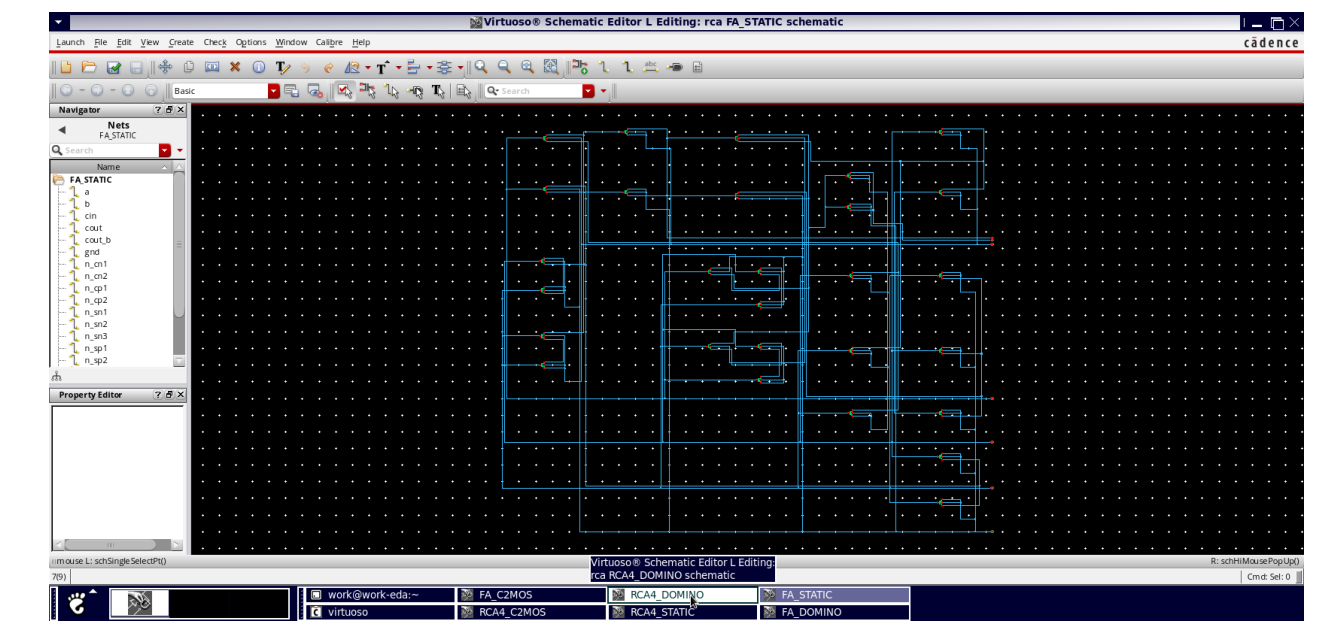
\includegraphics[width=.88\textwidth,height=.43\textheight,keepaspectratio]{../../assets/schematics/static/fa_static_schematic.png}\caption{Static CMOS one-bit full-adder transistor schematic.}\end{figure}
\begin{figure}[p]\centering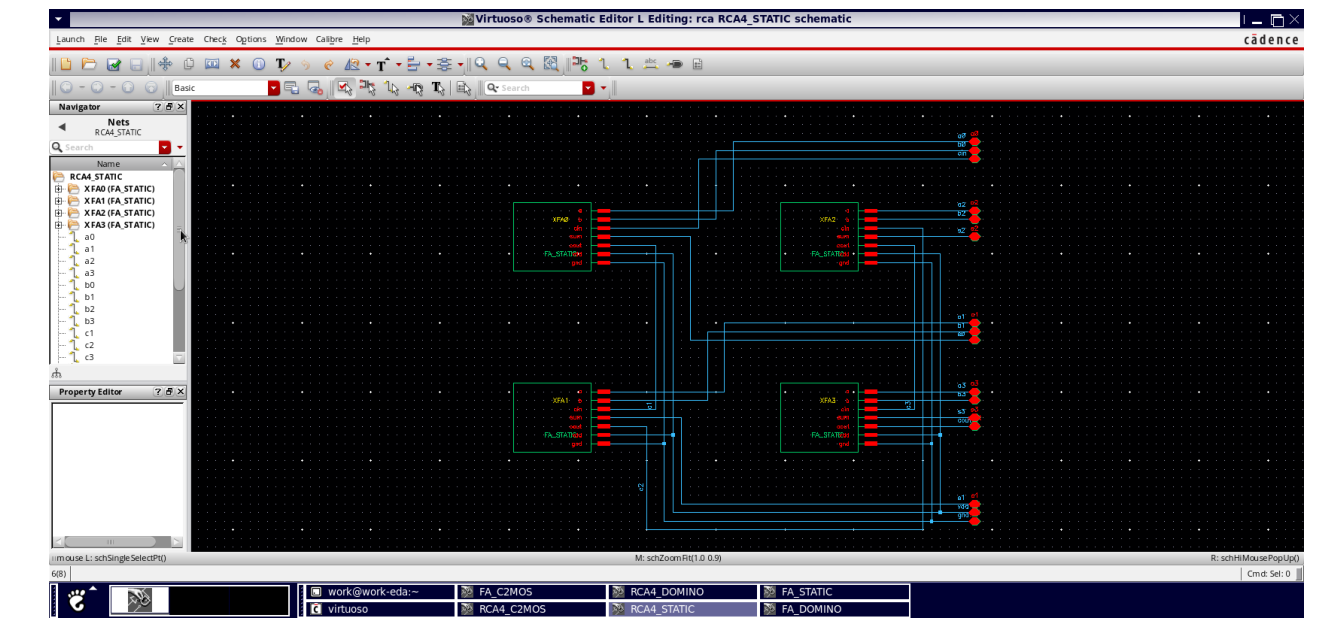
\includegraphics[width=.88\textwidth,height=.43\textheight,keepaspectratio]{../../assets/schematics/static/rca4_static_schematic.png}\caption{Four-stage Static CMOS ripple-carry adder.}\end{figure}
\begin{figure}[p]\centering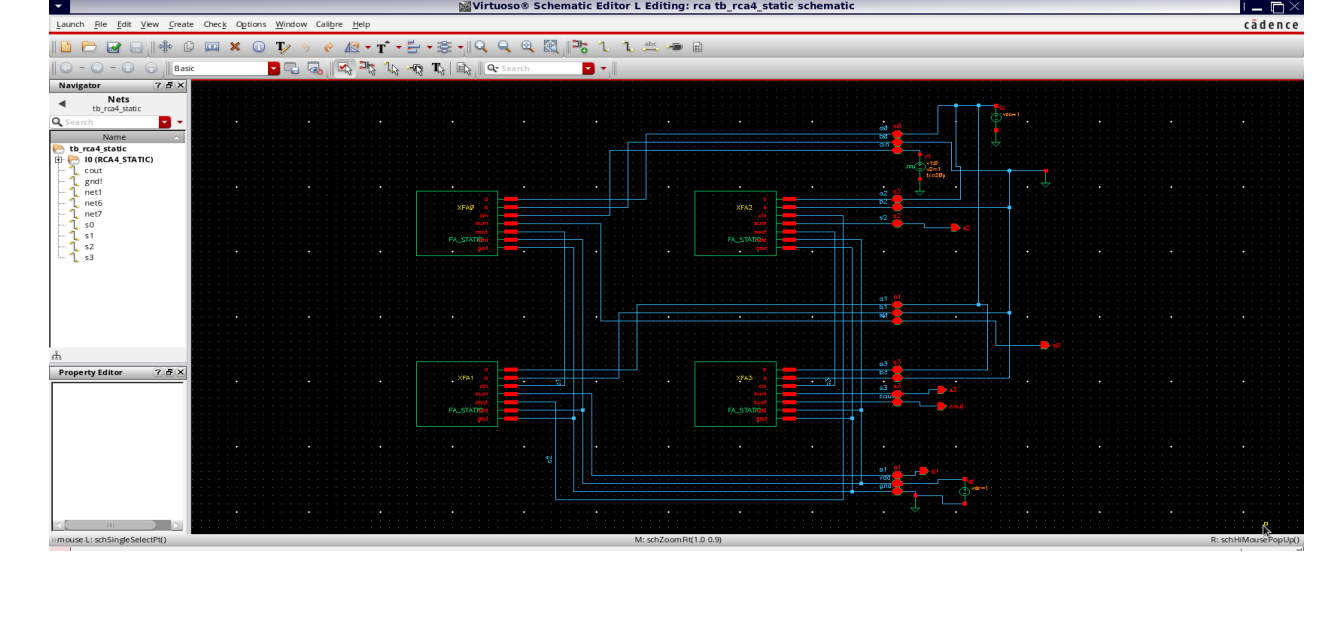
\includegraphics[width=.88\textwidth,height=.43\textheight,keepaspectratio]{../../assets/schematics/static/tb_static_schematic.png}\caption{Static CMOS simulation testbench.}\end{figure}
\begin{figure}[p]\centering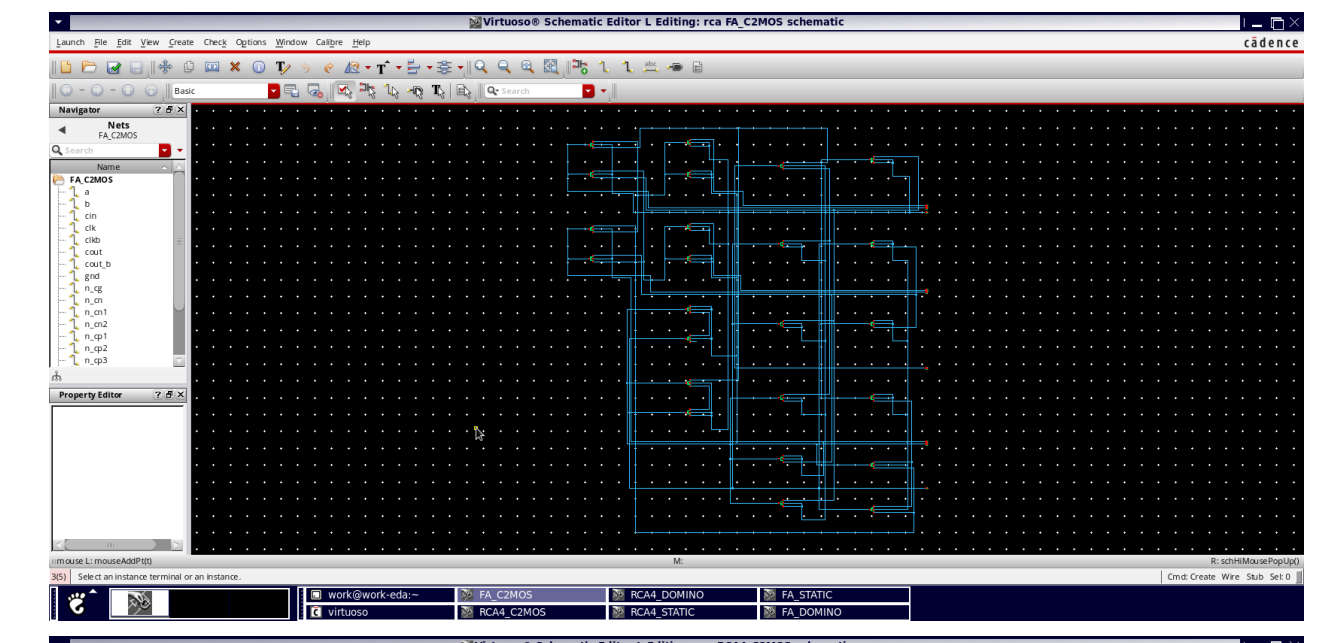
\includegraphics[width=.88\textwidth,height=.43\textheight,keepaspectratio]{../../assets/schematics/c2mos/fa_c2mos_schematic.png}\caption{C$^{2}$MOS one-bit full-adder transistor schematic.}\end{figure}
\begin{figure}[p]\centering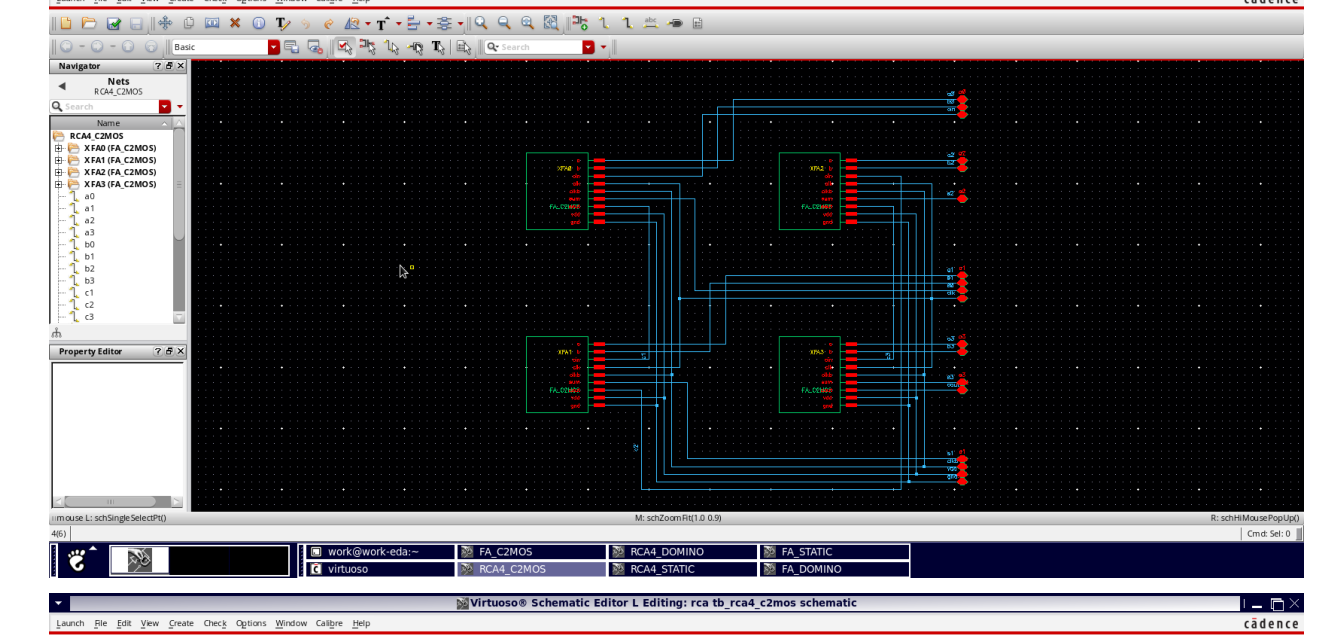
\includegraphics[width=.88\textwidth,height=.43\textheight,keepaspectratio]{../../assets/schematics/c2mos/rca4_c2mos_schematic.png}\caption{Four-stage C$^{2}$MOS ripple-carry adder.}\end{figure}
\begin{figure}[p]\centering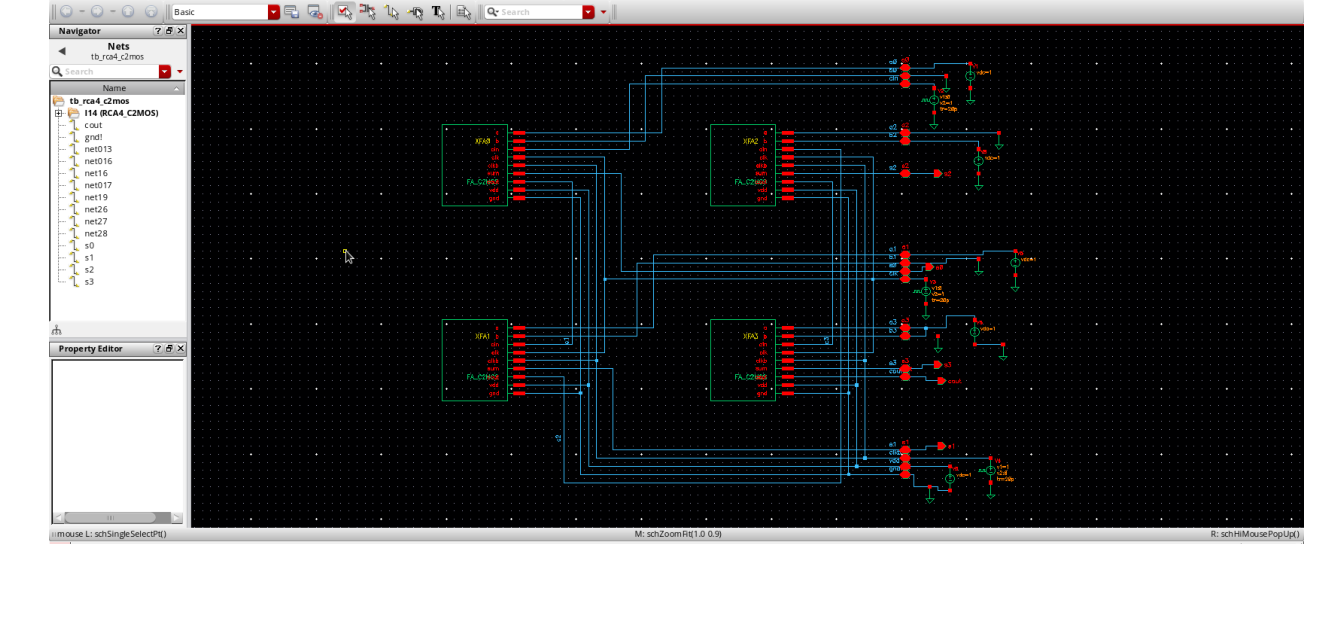
\includegraphics[width=.88\textwidth,height=.43\textheight,keepaspectratio]{../../assets/schematics/c2mos/tb_c2mos_schematic.png}\caption{C$^{2}$MOS simulation testbench.}\end{figure}
\begin{figure}[p]\centering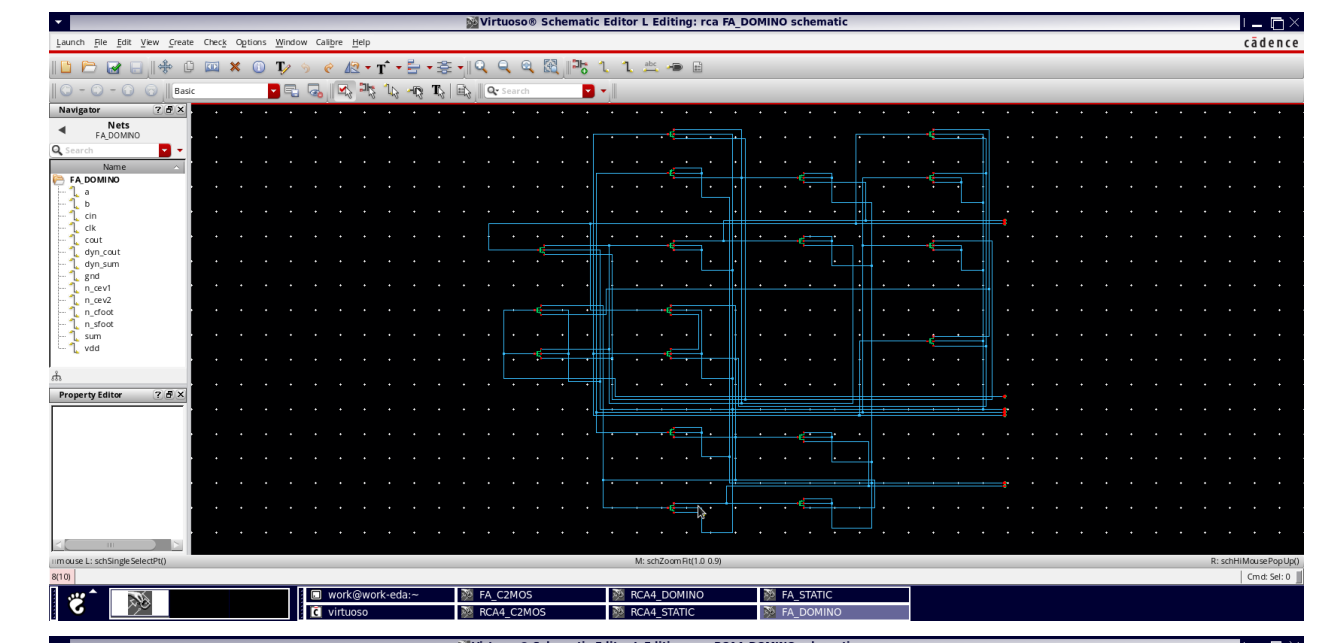
\includegraphics[width=.88\textwidth,height=.43\textheight,keepaspectratio]{../../assets/schematics/domino/fa_domino_schematic.png}\caption{Domino one-bit full-adder transistor schematic.}\end{figure}
\begin{figure}[p]\centering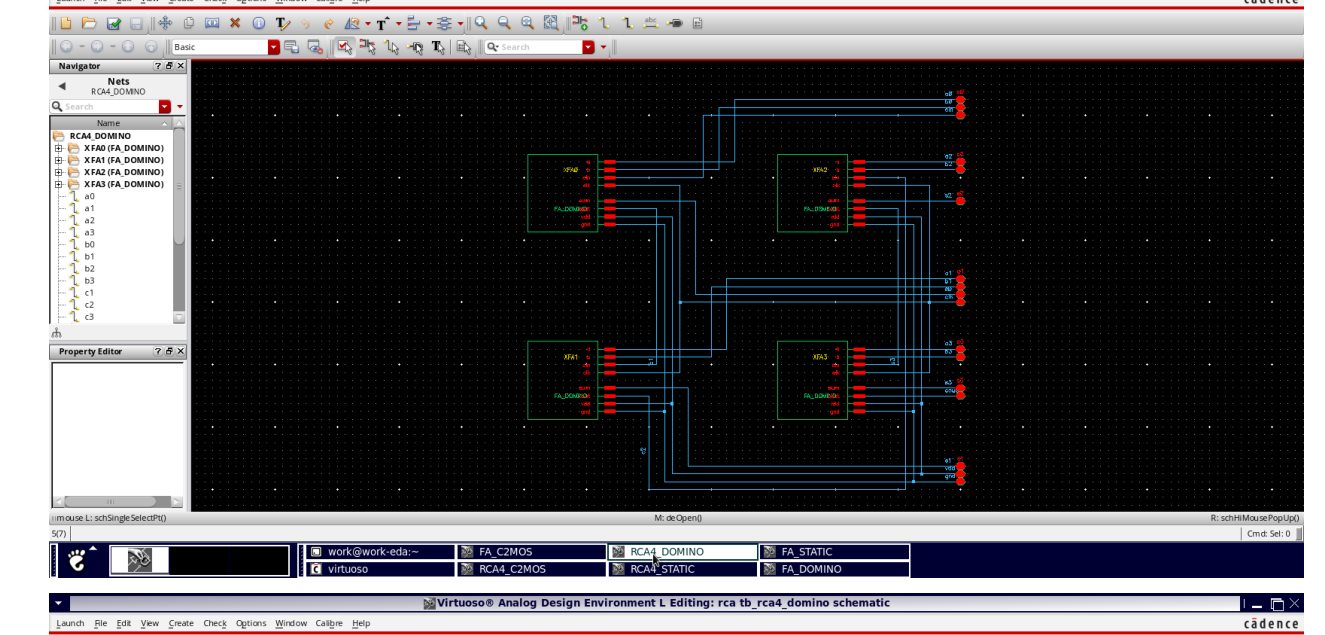
\includegraphics[width=.88\textwidth,height=.43\textheight,keepaspectratio]{../../assets/schematics/domino/rca4_domino_schematic.png}\caption{Four-stage Domino ripple-carry adder.}\end{figure}
\begin{figure}[p]\centering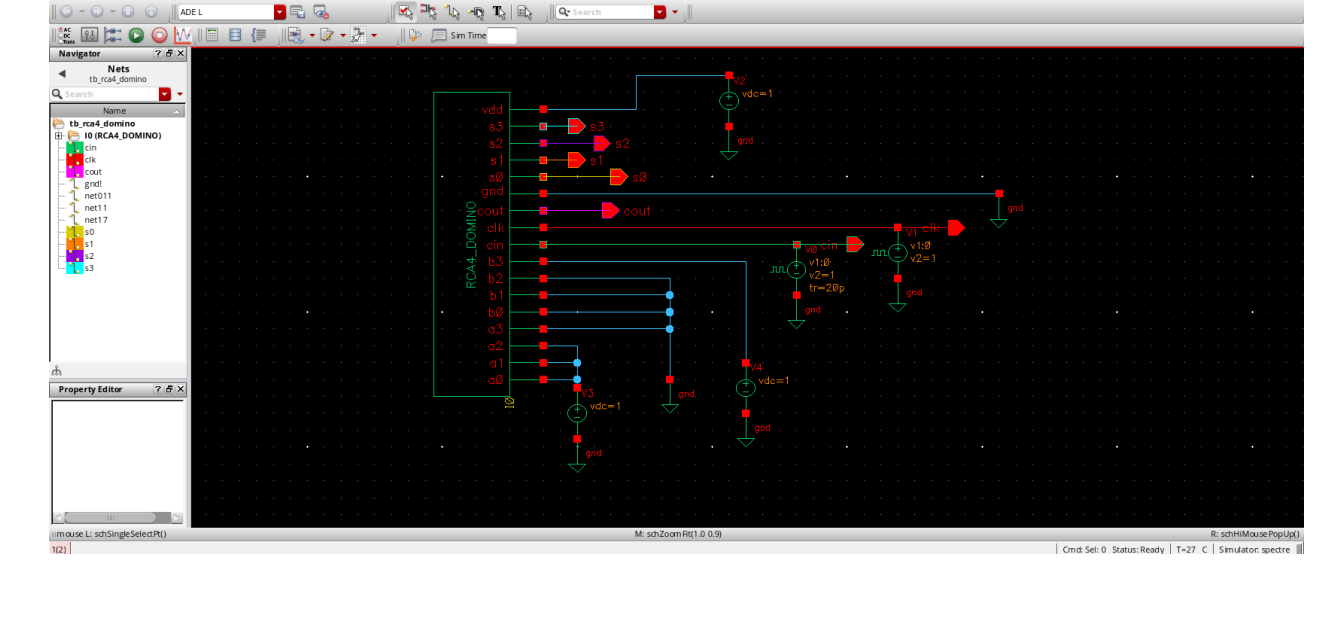
\includegraphics[width=.88\textwidth,height=.43\textheight,keepaspectratio]{../../assets/schematics/domino/tb_domino_schematic.png}\caption{Domino simulation testbench.}\end{figure}

\OutputFigure{../../assets/waveforms/static_output_waveforms.png}{Static CMOS output waveforms for the four-bit RCA.}
\OutputFigure{../../assets/waveforms/c2mos_output_waveforms.png}{C$^{2}$MOS output waveforms for the four-bit RCA.}
\OutputFigure{../../assets/waveforms/domino_output_waveforms.png}{Domino Logic output waveforms for the four-bit RCA.}

\section{Performance Parameters}
Power, delay, energy and area provide complementary views of a VLSI implementation. Average power combines switching, short-circuit and leakage components. Leakage power is the static component associated with off-state current, while dynamic power is associated with switching capacitance and frequency. Propagation delay measures the response from a defined input transition to an output transition. PDP is the product of average power and delay. Energy consumption is the integral of supply power over an operating interval. Transistor count is a circuit-complexity measure and a first-order area indicator; the physical layout also depends on device sizing and wiring.

The project calculator summaries report delay, average power and PDP for all three implementations. The PDP arithmetic checks as follows: 13.25 $\mu$W $\times$ 251.81 ps = 3.336 fJ; 29.49 $\mu$W $\times$ 260.75 ps = 7.689 fJ; and 30.76 $\mu$W $\times$ 222.35 ps = 6.839 fJ. These round to 3.34, 7.69 and 6.84 fJ.

The Static CMOS transition table records 248 ps from $C_{in}$ to $C_{out}$ and 265 ps from $C_{in}$ to $S_3$. The Domino waveform annotation gives 232 ps from $C_{in}$ to $S_2$. The C$^{2}$MOS simulation is represented by its reported calculator delay and clocked output transitions. These timing observations complement the reported calculator delays of 251.81 ps, 260.75 ps and 222.35 ps.

\begin{table}[htbp]
\centering
\caption{Performance parameters for the four-bit RCA implementations.}\small
\begin{tabularx}{\textwidth}{l c c c X}
\toprule Logic family & FA count; four-stage count & Calculator delay & Average power; PDP & Transient timing observation\\
\midrule
Static CMOS & 28; 112 & 251.81 ps & 13.25 $\mu$W; 3.34 fJ & $C_{in}\!\to C_{out}$: 248 ps; $C_{in}\!\to S_3$: 265 ps\\
C$^{2}$MOS & 32; 128 & 260.75 ps & 29.49 $\mu$W; 7.69 fJ & Clocked output transitions across carry-in intervals\\
Domino Logic & 26; 104 & 222.35 ps & 30.76 $\mu$W; 6.84 fJ & $C_{in}\!\to S_2$: 232 ps\\
\bottomrule
\end{tabularx}\end{table}
The transistor counts show the relative cell-level hardware complexity of the three implementations. Static CMOS uses 16.7\% more listed devices than Domino, and C$^{2}$MOS uses 33.3\% more. These device-count differences frame the area trade-off; the reported power and delay values describe the simulated circuit behavior.

Figure~\ref{fig:pdp-comparison} compares PDP values calculated from the reported average power and calculator delay. Static CMOS has the lowest PDP (3.34 fJ), while C$^{2}$MOS has the highest (7.69 fJ). Figure~\ref{fig:delay-comparison} shows that Domino has the lowest reported calculator delay at 222.35 ps. Figure~\ref{fig:power-comparison} shows that Static CMOS has the lowest reported average power at 13.25 $\mu$W.

\begin{figure}[htbp]
\centering
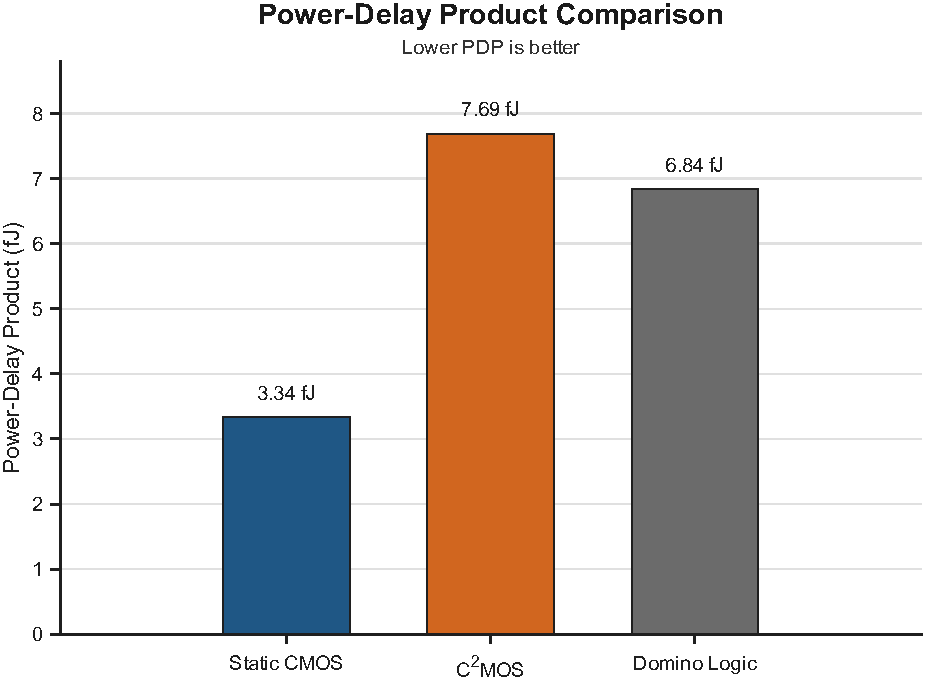
\includegraphics[width=.88\textwidth]{../../assets/plots/pdp_comparison.pdf}
\caption{Power-delay product calculated from the reported average power and calculator delay for each four-bit RCA implementation.}
\label{fig:pdp-comparison}
\end{figure}

\begin{figure}[htbp]
\centering
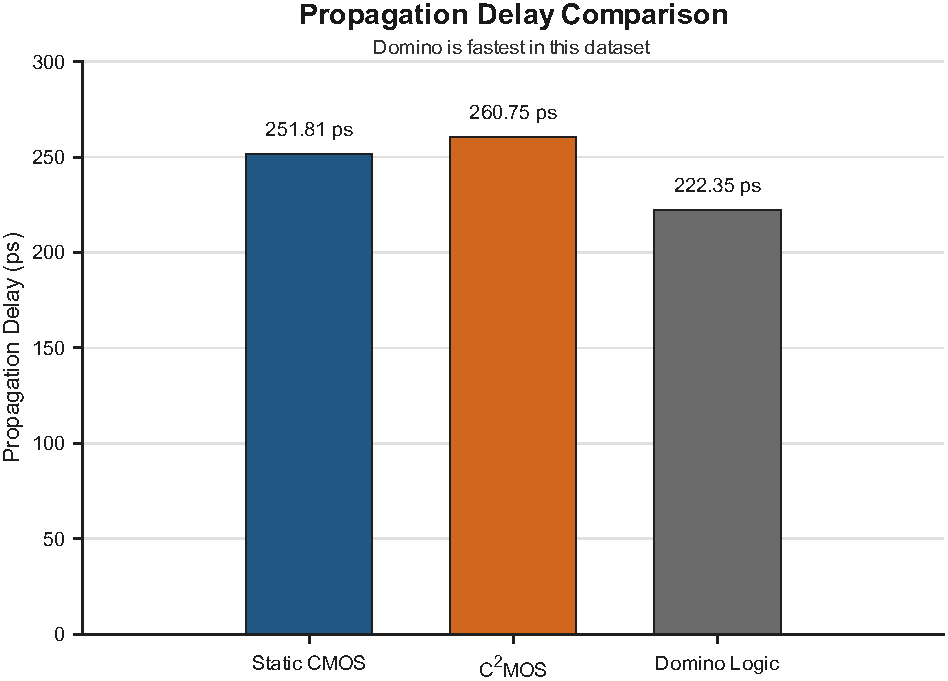
\includegraphics[width=.88\textwidth]{../../assets/plots/delay_comparison.pdf}
\caption{Reported calculator delay for the three four-bit RCA implementations; Domino has the lowest value in this dataset.}
\label{fig:delay-comparison}
\end{figure}

\begin{figure}[htbp]
\centering
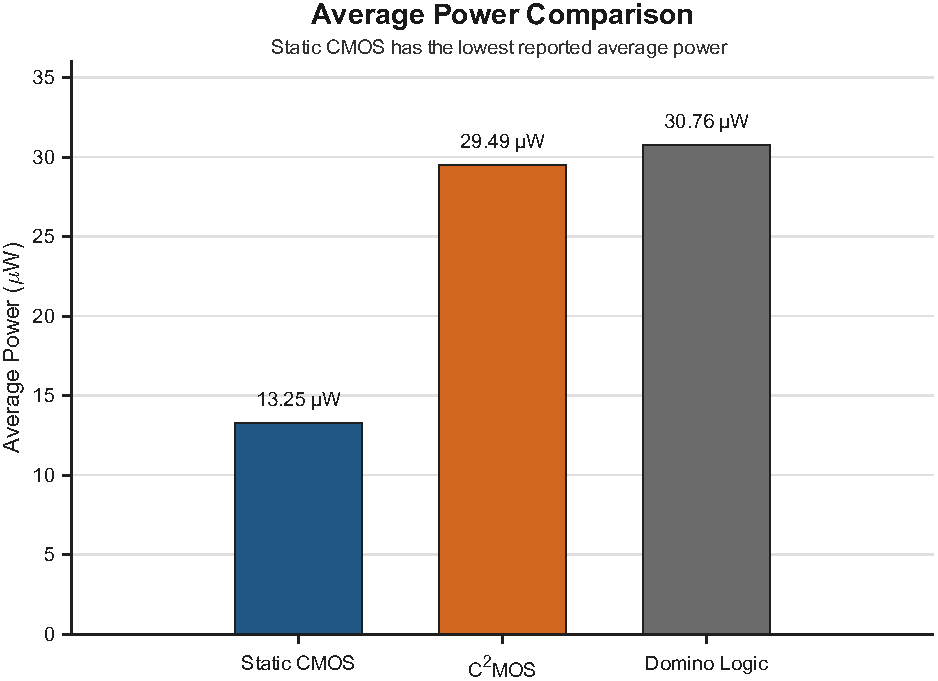
\includegraphics[width=.88\textwidth]{../../assets/plots/power_comparison.pdf}
\caption{Reported average power for the three four-bit RCA implementations; Static CMOS has the lowest value in this dataset.}
\label{fig:power-comparison}
\end{figure}

\section{Comparative Discussion}
As shown in Figures~\ref{fig:pdp-comparison}--\ref{fig:power-comparison}, the project calculator results place Static CMOS at 251.81 ps, 13.25 $\mu$W and 3.34 fJ PDP; C$^{2}$MOS at 260.75 ps, 29.49 $\mu$W and 7.69 fJ; and Domino Logic at 222.35 ps, 30.76 $\mu$W and 6.84 fJ. For this measurement set, Domino has the lowest reported delay, Static CMOS has the lowest reported average power and PDP, and C$^{2}$MOS has the highest reported PDP. These rankings describe these particular implementations and measurements, not universal properties of the logic families. Static CMOS's complementary networks provide full output restoration without an evaluation clock. C$^{2}$MOS and Domino introduce clocked operation, which supports phase-based evaluation but adds clock activity to the design.

Domino has the fewest listed transistors per FA (26: 11 PMOS and 15 NMOS), offering a compact cell-level implementation. In this case, the lower count does not coincide with the lowest average power: its reported 30.76 $\mu$W is the largest of the three. This illustrates why power cannot be inferred from transistor count alone; precharge/evaluation activity, switched capacitance and clock frequency also matter. The reported calculator delay for Domino is the lowest of the three implementations.

Reliability and noise behavior also influence architecture choice. Static CMOS restores outputs through complementary networks. C$^{2}$MOS depends on well-timed clock phases. Domino's dynamic nodes are sensitive to leakage, charge sharing, noise and process variation, so keeper design and clock sequencing are important. Published work on Domino variation and keeper techniques addresses these concerns, while transistor sizing and layout-aware studies show that power-delay results depend on design choices \cite{Alioto2008,Alioto2002,Zeydel2010,Garg2018}. The practical choice therefore depends on whether the target prioritizes low PDP, a compact cell, clocked sequencing or high-speed evaluation under the intended operating conditions.

\section{Research Gap}
The literature covers logic-style benchmarks, alternative FA cells, wide adders and Domino noise/variation mitigation. It also shows that full-adder behavior changes when the cell is cascaded and that energy-delay optimization can involve algorithm, transistor sizing and wiring together. A useful research opportunity is a matched comparison of Static CMOS, C$^{2}$MOS and Domino in the same RCA structure with aligned operand patterns and named endpoints, while measuring clock energy and data energy separately. This would connect the device-level differences reviewed in the literature to the carry-chain behavior of a complete arithmetic block.

\section{Future Scope}
Future work can extend the four-bit designs to larger word lengths and evaluate both carry transition polarities over targeted propagate and generate vectors. A common supply, loading and sizing plan would permit consistent delay, average-power and PDP comparison. Layout implementation can add extracted area and interconnect parasitics to the transistor-level results. C$^{2}$MOS studies can explore clock frequency and phase relationships; Domino studies can examine keeper sizing, noise tolerance and dynamic-node retention. PVT and Monte Carlo analysis would extend the comparison to variability and reliability. These directions build directly on the three implemented architectures and the published techniques summarized above.

\section{Conclusion}
This case study examined a four-bit ripple-carry adder in Static CMOS, C$^{2}$MOS and Domino Logic. The basic FA equations establish the carry path, while transistor-level schematics and the supplied transient output waveforms connect logic behavior to the three implementation styles. C$^{2}$MOS and Domino produce the expected outputs for their displayed arithmetic vectors, and the Static CMOS waveform shows ordered response to carry-in transitions.

Across the three implementations, the Cadence netlist gives 28, 32 and 26 MOSFETs per FA, calculator delays of 251.81 ps, 260.75 ps and 222.35 ps, average powers of 13.25, 29.49 and 30.76 $\mu$W, and PDP values of 3.34, 7.69 and 6.84 fJ. Domino gives the lowest reported calculator delay and the lowest FA transistor count; Static CMOS gives the lowest reported power and PDP. The literature review shows why these outcomes should be read as a trade-off among power, delay, area and reliability rather than as one universal ranking.

The central finding is that a compact dynamic cell and a low-power implementation are not synonymous: the Domino design reduces the reported per-cell transistor count, while Static CMOS leads the reported average-power and PDP comparison. A larger matched study of carry chains, clock costs and reliability can extend these results to practical arithmetic datapaths.

\section{References}
\renewcommand{\refname}{}
\bibliographystyle{IEEEtran}
\bibliography{references}
\end{document}
